\chapter{Uploading Facebook Reels for Reach}

This chapter follows a short School of Hard Knocks tutorial on uploading a Facebook Reel and packaging it for reach. The lecture is not a mathematical derivation in the physics sense; it is a procedural demonstration. Still, the useful structure is precise: choose the page, create the Reel, select the video, attach a sound layer, choose a cover, write a description, add relevant hashtags, and share. The chapter preserves that order while separating the speaker's concrete steps from his experiential claims about exposure. This material is curated by LazyingArt LLC with Video2Book.

\section{The Tutorial as a Sequence}

Josh begins by defining the task: upload to Facebook Reels and get as much exposure as possible from the post. The promise is deliberately narrow. We are not building a general theory of social media distribution; we are following a sequence of choices that can be repeated.

A compact way to write the workflow is
\begin{equation}
\mathcal{W}
=
(P,\ R,\ V,\ S,\ C,\ D,\ H,\ \mathrm{Share}),
\end{equation}
where \(P\) is the selected page, \(R\) is the Reel creation path, \(V\) is the video asset, \(S\) is the sound layer, \(C\) is the cover, \(D\) is the description, and \(H\) is the hashtag set. This notation is only bookkeeping. It does not claim that Facebook's ranking system is known from the lecture.

The opening also removes a small practical uncertainty. Josh says the process is the same on mobile and desktop, but he demonstrates on mobile. That matters because the visual evidence later shows the mobile ``New Reel'' composer, not a desktop upload page.

\section{From Page Selection to Video Selection}

The first operational move is identity. We do not merely upload a video somewhere on Facebook; we first choose the page under which the Reel will live. In the lecture the page is School of Hard Knocks. The steps are simple: log in, go to pages, select the intended page, find the place to create a post, and choose to create a Reel.

Once the Reel path is open, the next object is the video asset itself. Josh selects a clip described in the transcript as asking a social media expert and influencer for advice. At this stage the content is fixed enough that the remaining choices are packaging choices: sound, cover, description, hashtags, and the final share.

The resulting package can be summarized as
\begin{equation}
\mathrm{Reel\ package}
=
\mathrm{video}
+
\mathrm{sound\ layer}
+
\mathrm{cover}
+
\mathrm{description}
+
\mathrm{hashtags}.
\end{equation}
The point of writing it this way is not to formalize a platform algorithm. It is to keep the lecture's practical architecture visible: the same video can be surrounded by different discovery and conversion signals.

\begin{figure}
\centering
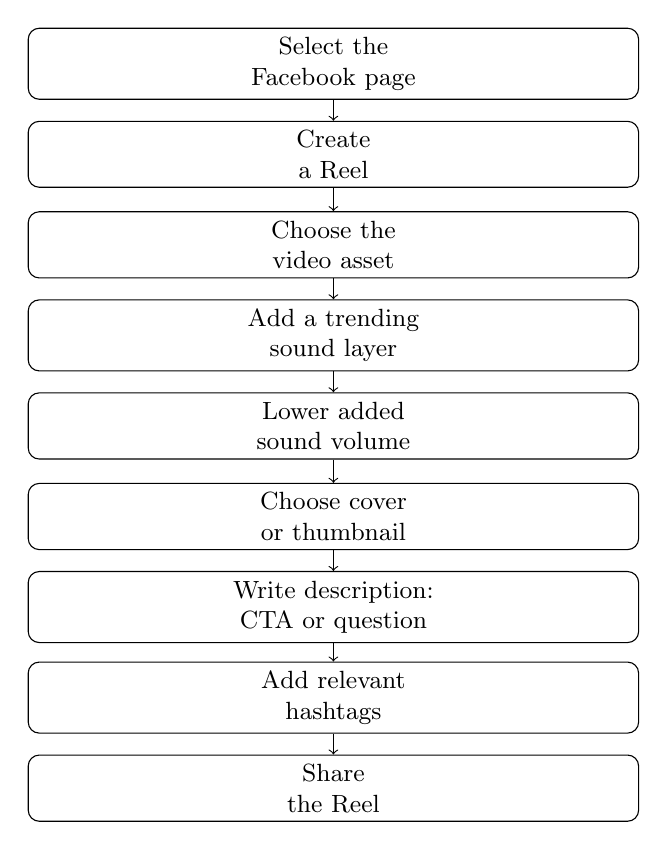
\begin{tikzpicture}[
  box/.style={draw, rounded corners, align=center, text width=0.62\linewidth, minimum height=0.62cm},
  every node/.style={font=\small}
]
\node[box] (p) at (0,0) {Select the\\Facebook page};
\node[box] (r) at (0,-1.15) {Create\\a Reel};
\node[box] (v) at (0,-2.30) {Choose the\\video asset};
\node[box] (s) at (0,-3.45) {Add a trending\\sound layer};
\node[box] (m) at (0,-4.60) {Lower added\\sound volume};
\node[box] (c) at (0,-5.75) {Choose cover\\or thumbnail};
\node[box] (d) at (0,-6.90) {Write description:\\CTA or question};
\node[box] (h) at (0,-8.05) {Add relevant\\hashtags};
\node[box] (x) at (0,-9.20) {Share\\the Reel};
\draw[->] (p) -- (r);
\draw[->] (r) -- (v);
\draw[->] (v) -- (s);
\draw[->] (s) -- (m);
\draw[->] (m) -- (c);
\draw[->] (c) -- (d);
\draw[->] (d) -- (h);
\draw[->] (h) -- (x);
\end{tikzpicture}
\caption{A narrow reconstruction of the spoken upload workflow. The diagram is transcript-derived; it is not a visible board diagram.}
\end{figure}

\section{The Sound Layer}

After selecting the video, Josh introduces the first real optimization claim. He says that, from his experience on TikTok and content creation, adding a sound tends to get videos more exposure. He then chooses a trending sound or artist. The lecture names ``Whoa'' by Lil Baby as the example.

We should state the claim carefully. In informal notation, let \(E\) denote exposure and let \(S\) denote the presence of an added sound layer. The lecture supports only the directional, anecdotal statement
\begin{equation}
\Delta E(S) > 0
\qquad
\text{as Josh's reported experience, not a measured law.}
\end{equation}
This equation is a reading aid. It should not be presented as a platform guarantee.

\subsection{Question \& Answer}

\paragraph{Question.}
Why add music if we do not actually want the audience to hear that music?

\paragraph{Answer.}
Josh separates the sound layer as a platform signal from the audio the viewer mainly hears. He adds the trending sound, then turns its volume down so the original video remains the dominant audible content. In a compact model, if \(A_0\) is the original video audio and \(A_{\mathrm{trend}}\) is the added sound, the tactic is
\begin{align}
A_{\mathrm{heard}} &= A_0 + \epsilon A_{\mathrm{trend}}, \\
0 &< \epsilon \ll 1, \\
\mathrm{package} &\text{ still contains the trending sound layer.}
\end{align}
The notation is ours; the tactic is his. The useful distinction is between what the platform may associate with the Reel and what the viewer primarily hears.

\section{Cover, Description, and the Composer Screen}

Once the sound is attached and lowered, Josh moves to the cover. The transcript is slightly uneven around the timeline and cover transition, but the reliable sequence is that he chooses the cover frame, goes next, and arrives at the Reel composer.

\begin{figure}
\centering

\includegraphics[width=0.62\linewidth]{lecture_177_figure_02.png}
\caption{Facebook's New Reel composer, with the description field open and Public visibility selected.}
\end{figure}

The screenshot shows the moment at which the video package becomes a publishing package. The field says ``Write a description...''; the visibility section asks who can see the Reel; ``Public'' is selected; and the keyboard is open. The image does not show the final description text, so the description advice comes from the transcript rather than from the screenshot.

Josh's description rule is simple. Use the description for a call to action or a thought-provoking question. His own leaning in this lecture is toward a call to action that asks people to follow for more content like this. The local mechanism is not mysterious: the description is a place to convert attention into a next action.

We can summarize the description choice as
\begin{equation}
D \in
\{\mathrm{call\ to\ action},\ \mathrm{thought\ provoking\ question}\}.
\end{equation}
Josh prefers the first option in this example, but he immediately widens the rule: experiment with different phrases, questions, and calls to action, then observe what gets traction.

\section{Hashtags and Niche Fit}

After the call to action, Josh adds hashtags. The important point is relevance on two levels. Some hashtags should match the particular post, such as social media or influencer for the selected clip. Others should match the page's broader niche, such as business, entrepreneur, finance, or related terms for School of Hard Knocks.

The one numerical guideline in the lecture is the count:
\begin{equation}
H \approx 6\text{--}7.
\end{equation}
Here \(H\) denotes the number of hashtags Josh says he typically uses. This is not a theorem about optimal hashtag count. It is a reported operating habit.

Putting the description and hashtags together, the packaging layer has two jobs:
\begin{align}
D &: \text{turn attention into an action or continued watching}, \\
H &: \text{mark topic and niche relevance}.
\end{align}
That distinction is useful because it prevents us from treating every caption element as doing the same work.

\section{Sharing and the Broader Strategy}

The final mechanical step is to press share. Once the Reel is posted, Josh closes by moving from the specific upload to a wider brand idea. Facebook Reels should be one part of the overall brand strategy, a way to build awareness around the brand rather than the whole strategy by itself.

A cautious reconstruction of the closing claim is
\begin{equation}
\mathrm{brand\ awareness}
\leftarrow
\mathrm{consistent\ publishing\ across\ social\ channels}.
\end{equation}
Again, this is not a measured equation. It is a compact way to record the strategic direction of the ending: use Facebook Reels as one repeatable content surface inside a broader system.

\section{Summary}

The lecture gives us a repeatable upload path and a small set of packaging levers. First we choose the page and create the Reel. Then we select the video, add a sound layer, reduce its audible volume, choose the cover, write a description, add relevant hashtags, and share.

The practical claims should remain source-conscious. The sound-layer tactic is Josh's reported experience, not a quantified rule. The hashtag count of six to seven is his operating habit, not a universal optimum. The most durable principle is the separation of roles: the video carries the content, the sound layer may help discovery, the cover frames the preview, the description asks for action, and the hashtags connect the post to its topic and niche.